% Chapter Template

\chapter{3D Models in Dentistry} % Main chapter title

\label{Chapter6} % Change X to a consecutive number; for referencing this chapter elsewhere, use \ref{ChapterX}

 %----------------------------------------------------
 
 
We discussed how to get a 3D digital model from diagnostic images and how to convert it into a physical model using 3D printing. Both the digital model and the physical model are elements that can elevate the quality of the therapies provided by the doctor, and at the same time are of great value for the clinical researcher for the amount of data obtainable.\\
The fields of application are many and embrace the surgical disciplines, education, dental procedures such as implantology, prosthetics and conservative \parencite{Reference103}.
We will discuss some of the most relevant implementations of the procedures we have described.

\section{Educazione}
\begin{wrapfigure} {R} {0.4\textwidth}
\vspace{-20pt}
	\begin{center}
	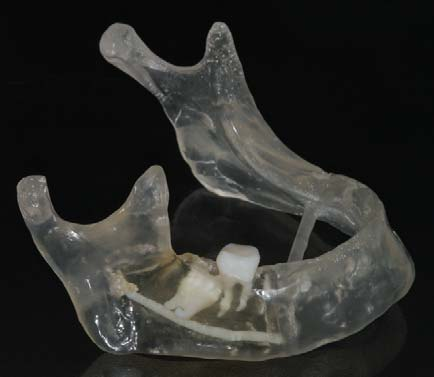
\includegraphics[width=0.4\textwidth, height=\textheight,keepaspectratio]{mandi_molar}
    \caption{modello3D ottenuto da CBCT, che presenta un terzo molare vicino al scondo molare, e con le radici in prossimità del nervo alveolare inferiore. Da \emph{Lambrecht et al} \parencite{Reference69}}
    \label{fig:mandi_molar}
    \end{center}
\vspace{-20pt}
\end{wrapfigure}
In the medical and dental degree courses the training path of the future professional is a combination of theoretical lessons and practical activities, aimed at providing in-depth medical knowledge and a method of clinical reasoning. Above all, the student has to develop manual skills to perform interventions on the patient. In addition, every student in the medical field studies the \emph{anatomy}, and if once the corpse dissections were what provided the students a context in which to apply what they had learned in books, now fewer and fewer institutes offer this possibility \parencite{Reference67}. \\
With the decrease in the use of cadavers, the use of plastic replicas of parts of the body has increased as a practical complement to the learning of anatomy. Several authors have recently begun to explore the possibilities offered by modern medical modeling and 3D printing techniques in the field of medical training. \\ Anatomical models and models have been produced for the explanation of operative procedures both in the medical and dental field \parencite{Reference66 }, \parencite{Reference70}. Heng \parencite{Reference67} evaluated the short-term improvement in an anatomical knowledge test for students, where 3D printed heart models and real cadaver hearts were used, positively evaluating the experience with 3D models. Lambrecht \parencite{Reference69} produced by means of a stereolithographic printer of the models of cases of extraction surgery to facilitate students the learning of complex surgical procedures \ref{fig: mandi_molar}.
\begin{figure}[h]
\vspace{-10pt}
	\begin{center}
	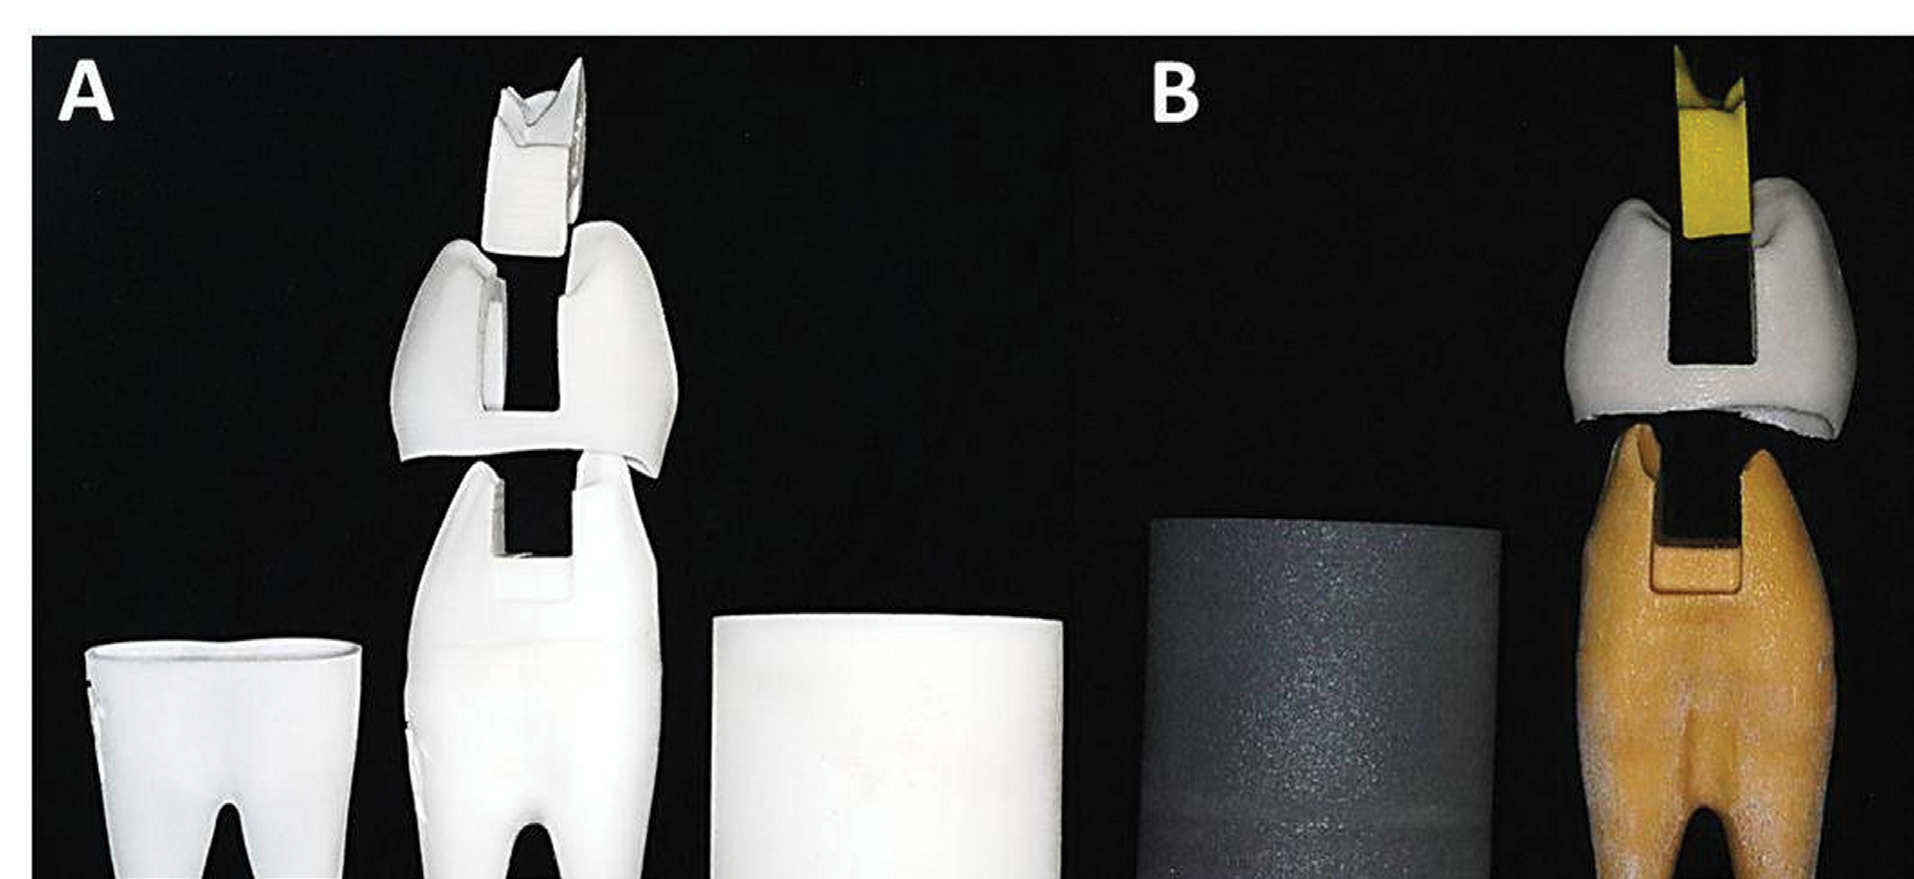
\includegraphics[width=0.8\textwidth, height=\textheight,keepaspectratio]{cavity_prep}
    \caption{Modelli dentali assemblabili rappresentanti delle preparazioni di cavità. Da \emph{Soares et al} \parencite{Reference71}}
    \label{fig:cavity_prep}
    \end{center}
\vspace{-20pt}
\end{figure}
 
Soares et al \parencite{Reference71} produced dental elements models prepared to instruct students on cavity preparation techniques \ref{fig: cavity_prep}. Other authors have realized 3D models as practical support for preclinical courses, for example Kroger et al \parencite{Reference72} has created models to perform caries removals and provisional fixtures; Reymus et al \parencite{Reference73} has printed replicas of dental elements with endodontic cavities to simulate endodontic preparation. The data common to these studies was the overall positive evaluation of the simulators printed in 3D by both the students and the teachers. 3D printers are also welcomed by students and university staff, as documented by Walker \parencite{Reference74}. \\
There are already several online libraries in which you can find anatomical models, such as the one provided by the \emph{NIH} \parencite{Reference75} and the one on the website \emph{Embodi3d} \parencite{Reference76}. Moreover, the possibilities offered by the workflow described here allow to create original anatomical models of complex cases or special procedures at reduced cost. The initial effort in the use of software is offset by the range of possibilities offered by the workflow in question as an aid to educating dentistry training.

\section{Programming of the surgical intervention}
Surgical planning is an important step in the treatment of the patient, because it provides the surgical team with an in-depth knowledge of the case under examination and allows to evaluate the best approach to surgery. The digital imaging techniques associated with 3D models have been experimented by several authors with the aim of providing the surgeon with a real reference to program the intervention. \\ Models that replicate the anatomy of the region to be operated have been created for different surgeries , from vascular surgery to orthopedic surgery. The \emph{Medical Modeling} book by Bibbs et al \parencite{Reference1} collects a series of interesting clinical, surgical, dental and research cases that show the use of medical modeling and rapid prototyping techniques. The surgeon can simulate on the models the execution of the osteotomies, simulate the new arrangement of the bone segments and create surgical guides as an aid to the intervention \parencite{Reference77}, \parencite{Reference78}.
\begin{figure}[h]
\vspace{-10pt}
	\begin{center}
	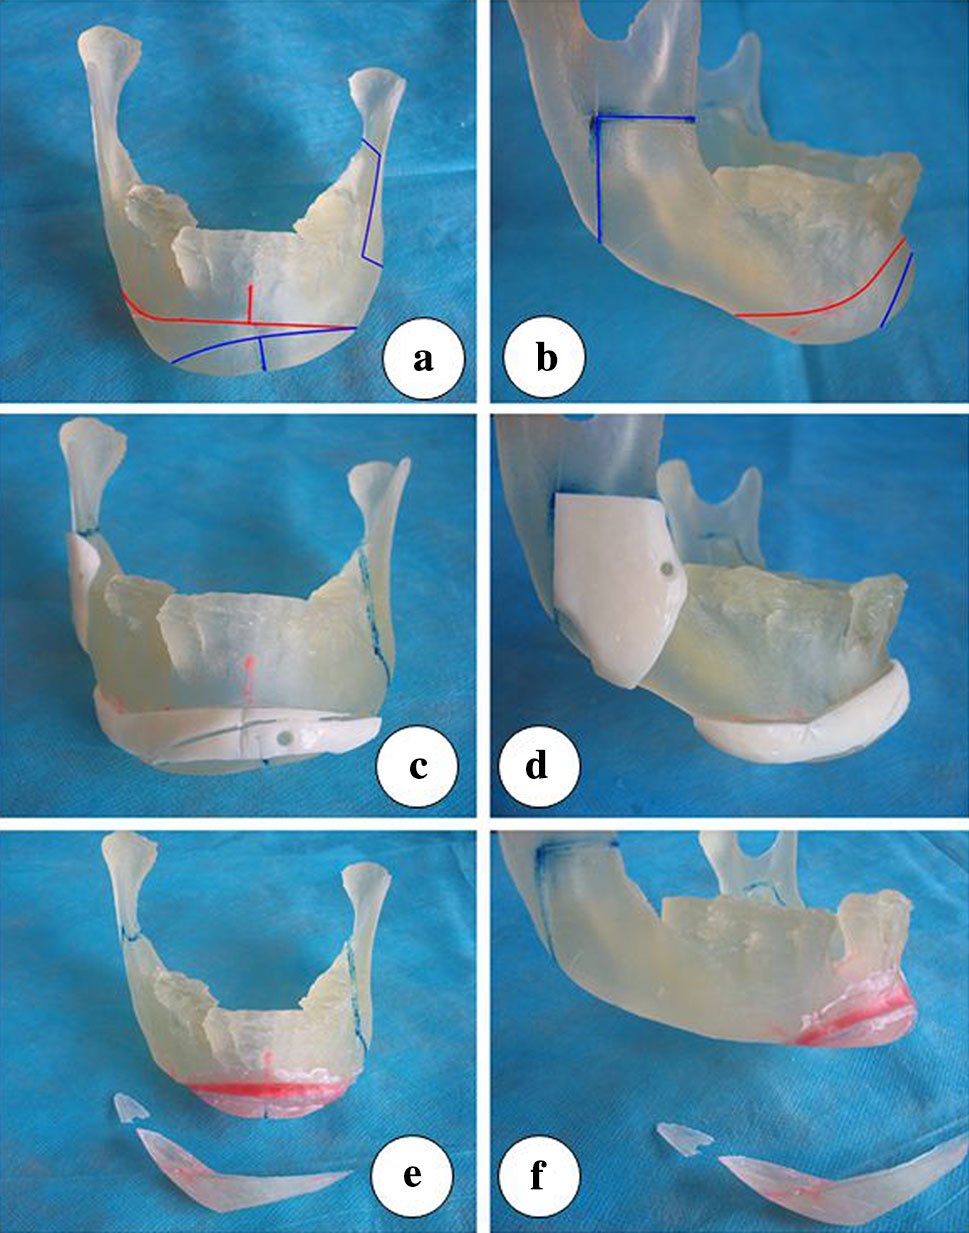
\includegraphics[width=0.5\textwidth,height=\textheight,keepaspectratio]{train_model}
    \caption{Modello per programmazione della chirurgia stampato in 3D.
\textbf{a}: Misure, analisi e linee di osteotomia marcate sul modello (vista frontale).\textbf{b}: Misure, analisi e linee di osteotomia marcate sul modello (vista laterale). \textbf{c}: Realizzazione del template chirurgico (vista frontale). \textbf{d}: Realizzazione del template chirurgico (vista laterale). \textbf{e}: Simulazione chirurgica (vista frontale). \textbf{f}: Simulazione chirurgica (vista laterale). Da \emph{Wang et al} \parencite{Reference20}.}
    \label{fig:train_model}
    \end{center}
\vspace{-20pt}
\end{figure}

For example, Wang \parencite{Reference109} reported the use of 3D models for the programming of mandibular orthognathic surgery and the manufacture of surgical guides, noting greater speed and precision in the execution of the osteotomy and repositioning of the bone segments \ref{fig:train_model}. \\
The Blender \emph{OrtogOnBlender} \parencite{Reference64}, \parencite{Reference79} plugin helps the programming of \emph{orthognathic surgery} \ref{fig:ortogon1}, facilitating the simulation of osteotomies and allowing to evaluate the consequences of bone mobilization on the patient's face. The patient's face can be scanned or detected with a series of photographs; OrtogOnBlender allows you to derive 3D models through photogrammetry, and to use these models in conjunction with the CT scans to make use of the models of the interior and exterior of the organism. In this way it is possible to simulate the consequences on the patient's face of the positioning of the bone segments \parencite{Reference145}.

\begin{figure}[h]
\vspace{-10pt}
	\begin{center}
	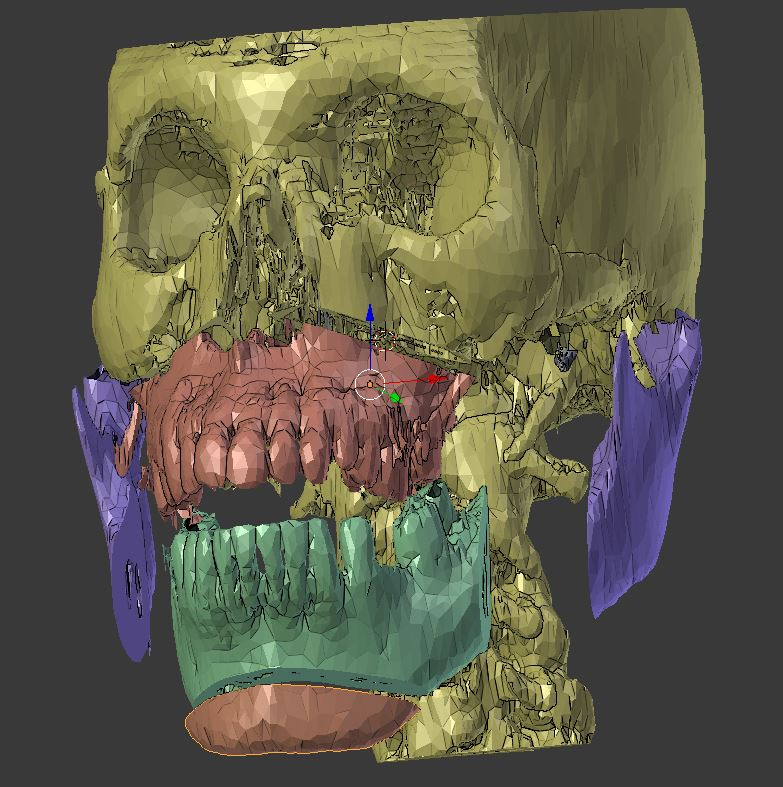
\includegraphics[width=0.6\textwidth,height=\textheight,keepaspectratio]{ortogon1}
    \caption{Osteotomie virtuali eseguite con add-on \emph{OrthogOnBlender}}
    \label{fig:ortogon1}
    \end{center}
\vspace{-20pt}
\end{figure}

The procedure for preparing orthognathic surgery simulation with OrtogOnBlender \parencite{Reference80} consists of loading DICOM images into Blender, but an already processed .stl model can also be used. The plugin facilitates the digital osteotomies by making available the cutting planes that are positioned in the desired position; perform the digital osteotomies we can isolate the segments and reposition them.
The management of the photos for the reconstruction in photogrammetry is very easy, just import the folder containing the photos and the software automatically creates the model of the patient's face. Through a few operations the scan of the face aligns with the images of the CT and it is possible to evaluate the virtualization of the jaws.
Rapid prototyping technologies have been used successfully for the realization of a custom surgical obturator following the removal of an upper maxillary carcinoma \parencite{Reference81}. \\
Ackland et al \parencite{Reference82} rehabilitated a patient with osteoarthritis at the \emph{Temporary Mandibular Articulation} (ATM) by designing a customized prosthesis, on which they performed computer mechanical simulations (FEA) to optimize their position and fixation . The digital model was then printed in Titanium 6Al4V with an SLS printer and implanted on the patient with good results. \\
The integration of digital techniques and 3D printing in the surgical workflow can be of considerable help to the surgeon for the preparation of the operation, especially in cases of complex surgeries and in sensitive areas of the organism (for example, near beams neurovascular). These technologies also allow to customize any rehabilitation devices, such as prostheses that adapt to the patient's anatomy and biomechanics. Multidisciplinary collaboration in surgical planning is a building block of this rehabilitative approach focused on personalization.


\section{Digital dentistry and 3D printing}

\subsection{Implant Surgical Guides}
Digital imaging is fundamental in implantology for implant site selection, while modeling and rapid prototyping techniques allow to quickly create customized surgical guides, which can be autoclaved and used for the insertion of the \parencite{Reference83} implants. As shown by literature analysis, the surgical guide allows to operate with greater precision than the manual insertion procedures of the implant. Van Assche \parencite{Reference105} carried out a literature review, giving indications on the use of surgical guides in implantology (Fig. 34). The position of the implant inserted with the guides is more predictable than the manual insertion, and the guide in the implant insertion phase has a higher precision than the guidance of the sole osteotomies, where only the site preparation is guided, while the subsequent insertion of the fixture is manual. The average error found with the guides is about 1mm in the entry position, 1.3mm at the apex and an angle difference of about 4 degrees, although with a wide variability between the studies analyzed.

\begin{figure}[h!]
 
\begin{subfigure}{0.5\textwidth}
\centering
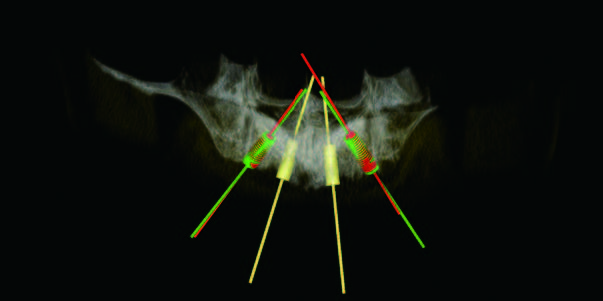
\includegraphics[width=0.9\linewidth, keepaspectratio]{beretta_digital} 
%\caption{Skirt}
\label{fig:beretta_digital}
\end{subfigure}
\begin{subfigure}{0.5\textwidth}
\centering
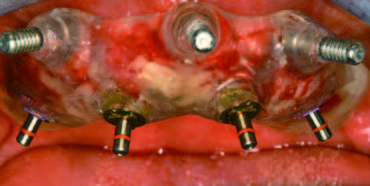
\includegraphics[width=0.9\linewidth, keepaspectratio]{beretta_real}
%\caption{}
\label{fig:beretta_real}
\end{subfigure}

\caption{\textbf{A sinistra}: Sovrapposizione tra simulazione degli impianti nella TC preoperatoria (rosso) e scansione postoperatoria con impianti inseriti (verde). \textbf{In basso}: Guida chirurgica per l'arcata madibolare, stabilizzata con miniimpianti. Da \emph{Beretta et al} \parencite{Reference104}.}
\label{fig:Beretta}
\end{figure}

Beretta \parencite{Reference104} has found similar data in the literature, but in its small series of 14 implant rehabilitations performed with surgical guides found lower errors. The greatest precision is attributed to some measures, such as the use of extraoral references for correct anatomical positioning, the combined use of CT scans and optical scans in positioning procedures, and intraoral fixation of the guide with mini implants \ref{fig:Beretta}. \\
According to the analyzed reports the use of the surgical guides is a valid aid to the implant insertion procedures, keeping in mind an adequate margin of error of at least 2mm from sensitive areas \parencite{Reference104}. The accuracy in the production of the guides is fundamental, so we must try to reduce the error accumulated between the operations of scanning the arches, design and manufacture of the guide.
 
\subsection{Root Analog Implants}
In the field of implantology, the authors described anatomical implants to be inserted in post-extraction alveoluses (Root Analog Implant). These implants are made with CAD / CAM techniques of additive or subtractive manufacturing (milling), and replicate the morphology of the dental element to be replaced. The anatomy of the alveolus can be obtained through the use of a CBCT scan or with the optical scan of the extracted tooth. The optical scan requires operating in two steps, there being the need to extract the tooth to scan it, create the digital model, print the implant and reopen the surgical site to insert it. The preoperative CBCT allows to plan the intervention, to create the personalized implant and then to insert it immediately after the extraction of the dental element, in a single session.
\begin{figure}[h]
\vspace{-10pt}
	\begin{center}
	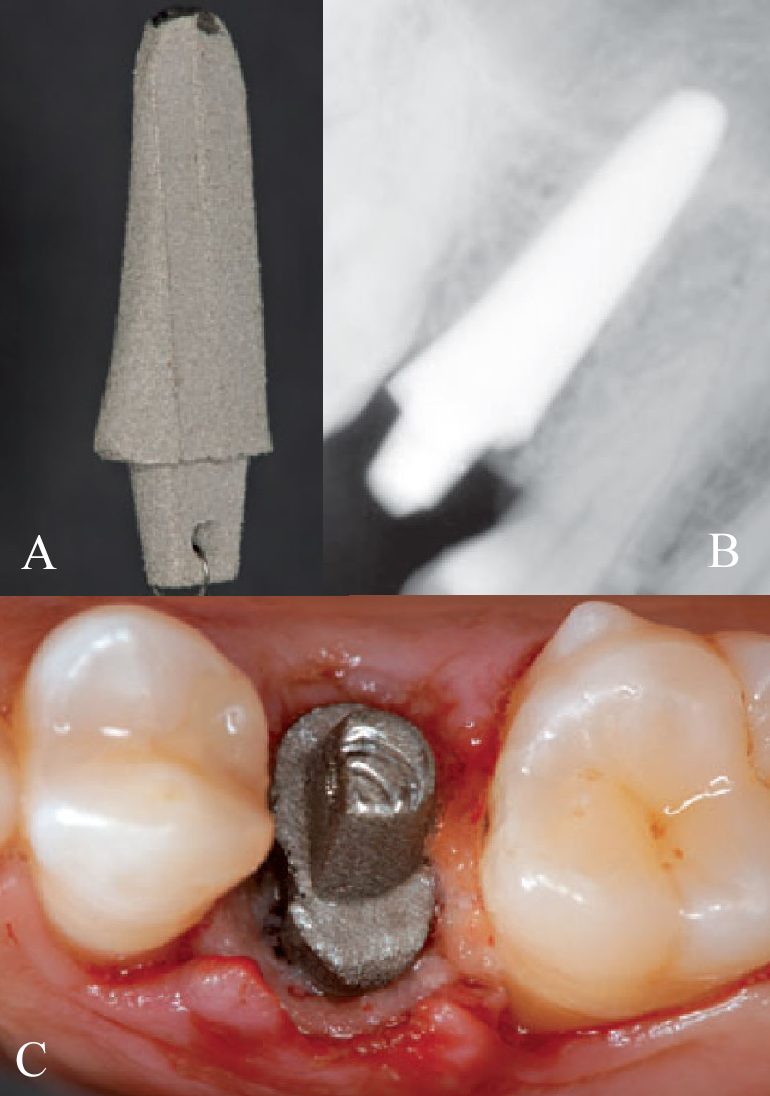
\includegraphics[width=0.5\textwidth,height=\textheight,keepaspectratio]{mangano_implant}
    \caption{Impianti anatomici realizzati con tecnologia DLMF. \textbf{A}: impianto anatomico in titanio. \textbf{B}: radiografia dell'impianto inserito in alveolo. \textbf{C}: aspetto clinico dell'impianto in cavo orale. Da \emph{Mangano et al} \parencite{Reference84}}
    \label{fig:mangano_implant}
    \end{center}
\vspace{-20pt}
\end{figure}

Mangano \parencite{Reference84} used CBCT reconstructions to make the system customized by means of DLMF (\emph{Direct Laser Metal Forming}) printing technology, which uses a laser to sinter titanium particle layers at a height of 0.2 mm \ref{fig:mangano_implant}. The implant was definitively prosthetised and the maintenance of peri-implant tissues was noted at the annual inspection.
Mangano \parencite{Reference85} then performed a study of 15 patients, using anatomical titanium implants. Although further studies are needed, the work showed how titanium anatomical implants made with DLMS (\emph{Direct Laser Metal Sintering}) can be a treatment option for post-extractive rehabilitation cases of dental elements where avulsion is possible atraumatica, where corticals are kept intact. \\
Pirker \ parencite {Reference86} modified the root of the extracted tooth with the addition of composite macro-concentrations on the distal and proximal portion, leaving the vestibular surface and the lingual surface of the root unaltered. The root thus modified was scanned with an optical scanner, and the obtained digital model was slightly reduced in the diameter of the vestibular region and of the lingual region (between 0.1 and 0.3 mm) to limit the risk of fracture of the alveolar cortices. The implant was then produced in zirconia using a CAD-CAM milling machine and implanted in the alveolus \ref{fig:bioimplant}. Primary stability was optimal, thanks to the use of interdental macroretention. At the 2 year follow-up there were no signs of bone resorption and gingival retraction, also sign of a correct distribution of stress on the alveolus wall.
\begin{figure}[h]
\vspace{-10pt}
	\begin{center}
	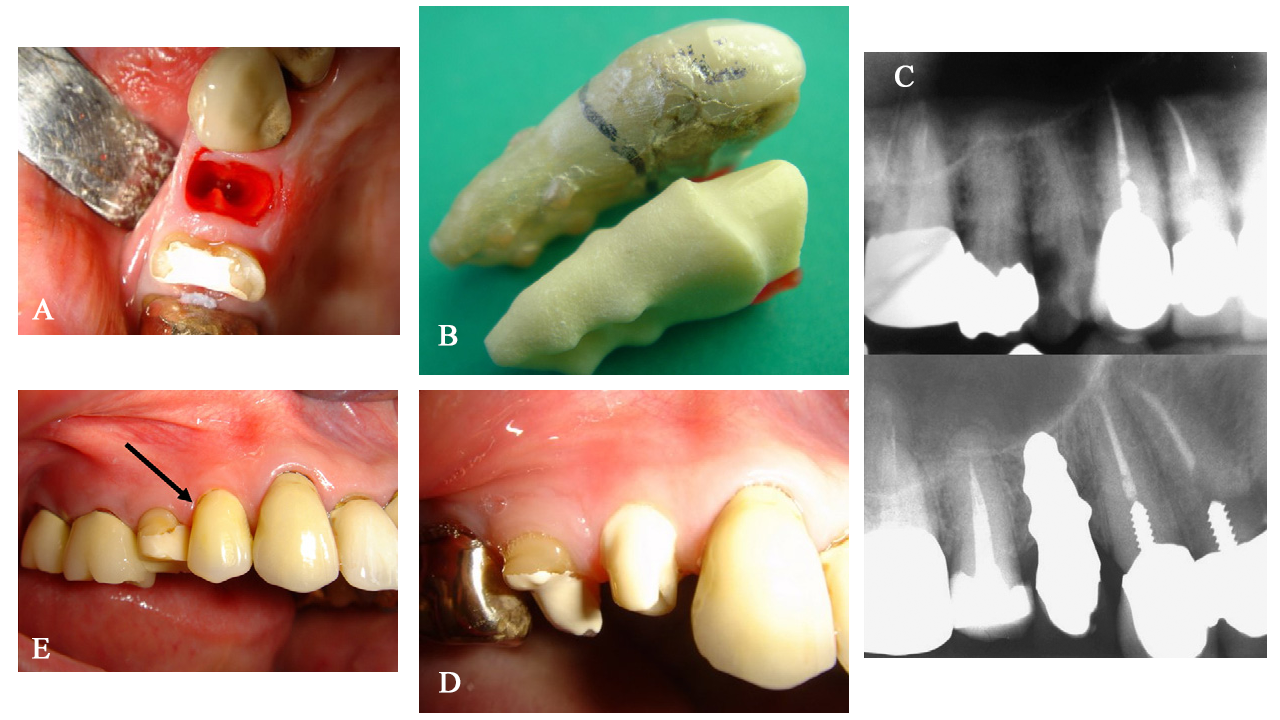
\includegraphics[width=0.9\textwidth,height=\textheight,keepaspectratio]{bioimplant}
    \caption{Inserimento e controllo impianto anatomico in zirconia. A: alveolo intatto di premolare estratto atraumaticamente. B: Elemento dentario estratto con ritenzioni simulate con composito, e impianto anatomico in zirconia con macroritenzioni. C: Radiografia pretrattamento (in alto) e post trattamento, con impianto anatomico inserito (in basso). D: impianto anatomico inserito. E: controllo clinico dopo 2 anni dall'inserimento dell'impianto; si nota il mantenimento dei tessuti parodontali. Da \emph{Pirker et al} \parencite{Reference86}}
    \label{fig:bioimplant}
    \end{center}
\vspace{-10pt}
\end{figure}

The same author then made a comparison between different topographies of anatomical zirconia implants made with CAD-CAM technology in a two group of patients \parencite{Reference87}. A group of patients was rehabilitated with anatomical implants with a rough surface created by sandblasting, while the second group was treated with sandblasted implants on which macroraintions on the interdental surfaces were present. The group of sandblasted implants showed a success rate of 0\%, with all 6 implants inserted that failed before being repaired. The group treated with plants with macro-absorption showed a success rate of 92\% at two years, with only one implant lost on 12 inserted. The failure of the microrentained implants was attributed to the uniform pressure exerted by the implant on the alveolus walls, but in case with macroritenzioni the distribution of the load in defined areas allowed to reduce the stress on the bone, favoring the osseointegration of the facility. \\
Patankar \parencite{Reference88} replicated the anatomic structure in zirconia of Pirker with interdental macroretentions, for the rehabilitation of a lower premolar, with a positive result.

\begin{wrapfigure} {R} {0.4\textwidth}
\vspace{-20pt}
	\begin{center}
	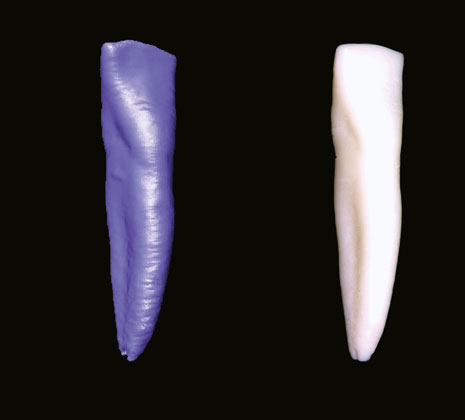
\includegraphics[width=0.4\textwidth, height=\textheight,keepaspectratio]{moin_dlp_zirconia}
    \caption{a sinistra modello CAD dell'elemento dentario. A destra modello dentario  in zirconia stampato stampato con tecnica DLP. Da \emph{Moin et al} \parencite{Reference89}}
    \label{fig:moin_dlp_zirconia}
    \end{center}
\vspace{-20pt}
\end{wrapfigure}

Moin \parencite{Reference89} used the Digital Light Processing (DLP) additive manufacturing technique to realize a zirconia replica of a dental element \ref{fig:moin_dlp_zirconia}. The author then digitally compared the CAD model of the replica, the scan of the printed zirconia replica and the scan of the original dental element, noting the adequate precision of the DLP technology for the additive manufacturing of zirconia products. \\
The production of ceramic artefacts is currently also possible using the extrusion printing technique, as documented by Nötzel \parencite{Reference97}. The process used consists in the production of a filament composed of paraffin, LDPE and Al2O3 particles; the filament is molded by extrusion to form the object, which is then subjected to chemical and thermal treatment for the removal of the medium in which the Al2O3 particles are dispersed and finally sintered in the oven to give the final product. The printing by extrusion of ceramic products is still to be evaluated in the field of production of dental products. \\

These reports show us that, using digital techniques, the production of anatomic implants is now possible in a precise manner and with the use of biomaterials that promote osseointegration and aesthetic and functional rehabilitation.\\
The correct determination of the alveolus morphology and of the replacement implant, and of the distribution of the masticatory forces on the alveolar bone, is important in this perspective. An atraumatic avulsion is at the basis of rehabilitation with anatomical implants, because any trauma to the alveolus results in bone resorption and gingival retractions, with consequent degradation of the aesthetic characteristics of the rehabilitation. The distribution of the forces on the alveolus is also to be observed. \\ With the anatomical implants we seek primary stability by means of the dimensional congruity between the alveolus and the anatomic implant; it has been shown that excessive stress on the alveolus walls causes implant failure, probably due to reduction of the blood supply to the implant site and to the surrounding bone, which undergoes reabsorption. Further studies are necessary to verify the safety and standardization of the procedures currently present, but the anatomical implants could allow, in selected cases, a functional and aesthetic solution to the patient problem, and facilitate the resolution of post-implantation cases maintaining high aesthetic standards.

\subsection{Protesi}
Rapid prototyping has been used both in fixed prostheses and in removable prostheses, for the realization of molded temporary restorations, aesthetic guides, mockups and for the realization of skeletons. Various additive manufacturing technologies and various materials were used. \\
Tahayeri \parencite{Reference98} has tested various features of SLA printing with specific resins for dental use (NextDent), evaluating the influence of some parameters on printing precision, on mechanical properties and on the degree of conversion of the resin. The printed specimens proved to be in the precision range required for clinical use, as were the mechanical properties of the samples themselves. The author has noticed differences between the characteristics in the printing of various dental resins made by the same manufacturer, as well as different intensities of the laser during the polymerization of the various resins, based on the more or less dark color of the resin and the relative light absorption rate . A selection of resins and printers optimized for joint use could further improve print accuracy; better results may result from the fine adjustment of the printer features being printed.
To be considered that, according to the manufacturer's indications, the resin would have had to undergo a second polymerization step after printing, which the authors did not perform to accelerate the eventual production process of the temporary. Nevertheless, the mechanical properties of the non-post-polymerized resin have proved to be adequate to resist intraoral loads. \\
Katreva \parencite{Reference99} realized a workflow that integrated the use of 3D printed working models, the 3D printing of the provisionals and the printing of the final prosthesis for the pressed ceramic conversion. \\
Revilla-León \parencite{Reference100} used a digital workflow for the scanning of impressions, the creation of the diagnostic wax-up, the printing of a guide for the realization of the provisionals and finally for the production of the veneers, useful for aesthetic and functional rehabilitation anterior sector of the maxillary arch. The guide for the construction of the provisionals was made using the DLP 3D printing technique, while the final lithium disilicate veneers were milled to the CAD-CAM. \\
Alharbi \parencite{Reference101} has evaluated the possibility of making prosthetic crowns with SLA printing technique. The author has measured the accuracy of the printed crown at various angles to the plane and with the use of different sizes of supports. The same research group then evaluated the accuracy in crown printing using the DLP \parencite{Reference102} printing technique. Both technologies proved to be accurate, with SLA printing, which showed greater accuracy in replicating the morphology of the digital model. Both technologies are interesting for use in dentistry, but it is necessary to carry out further studies on the influence of the printing parameters on the final model and deepen the properties of dental resins.
\begin{wrapfigure} {R} {0.4\textwidth}
\vspace{-20pt}
	\begin{center}
	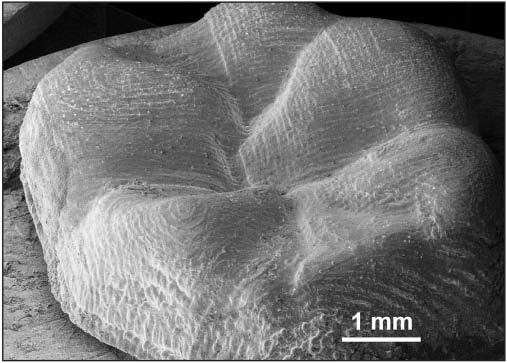
\includegraphics[width=0.4\textwidth, height=\textheight,keepaspectratio]{zircon_crown}
    \caption{Corona in zirconia realizzata con stampa ink-jet. Da \emph{Ebert et al} \parencite{Reference106}}
    \label{fig:zircon_crown}
    \end{center}
\vspace{-20pt}
\end{wrapfigure}

Ebert printed zirconia crowns using a custom printer, using the ink-jet technique. To make the crown, a zirconia-containing solution was deposited layer by layer to form the product, which was then sintered in the oven \ref{fig:zircon_crown}. This study has shown that zirconia crowns with mechanical abilities and precision useful for clinical use can be achieved by means of an additive ink-jet manufacturing technique \parencite{Reference106}. \\
Alharbi \parencite{Reference107} evaluated the use of additive manufacturing in prosthetics, analyzing various reports and studies focusing on the fixed prosthesis and the partial and total mobile prosthesis. The author has reported that the metal substructures realized with the SLS (\emph{Selective Laser Sintering}) method are equivalent or more precise than the classical fusion procedures regarding the gap between the metal substructure and the dental abutment; in the same way the mechanical properties of the SLS products were equivalent or better than those realized with the classical procedures. Metallic structures for the realization of removable partial dentures were produced by means of additive manufacturing either directly or indirectly. Direct manufacturing consists of printing the design by means of SLS processes; Indirect manufacturing consists in the realization of the castable resin product by means of SLA or DLP printing, the integration of the calcinable model in refractory material and the subsequent casting of the metal or alloy for the realization of the metallic framework. Both techniques for building removable prosthesis frameworks have shown acceptable accuracy, although the results are primarily derived from in vitro and case report studies. \\
Lin \parencite{Reference108} has demonstrated a technique for the realization of provisional total prostheses through a digital protocol that provides optical scanning, digital diagnostic waxing of the prosthesis, printing of the prosthetic base and respective dental arch in separate phases and with resins of color and suitable characteristics, and finally the union of arch and prosthetic base \ref{fig:separ_full_prot}. The study has not tested its use on the patient and there are no further reports of the clinical performance of total provisional removable prostheses made with this procedure and these materials. This concept could be explored, evaluating the accuracy compared to the other available manufacturing methods and the duration of the prosthesis over time, both from the point of view of color and wear of the resin.
The available data on digital treatment planning techniques and the use of additive manufacturing technologies show promising prospects in dentistry, both for the production of temporaries \parencite{Reference125} and of removable prostheses \parencite{Reference107}. Further studies and evaluations with longer follow-up are still necessary before extensive clinical application of the technology. Furthermore, the possibility of producing definitive ceramic or zirconia artefacts, possibly achievable with technologies such as SLS or inkjet printing, remains unexplored.
\begin{figure}[h]
\vspace{-10pt}
	\begin{center}
	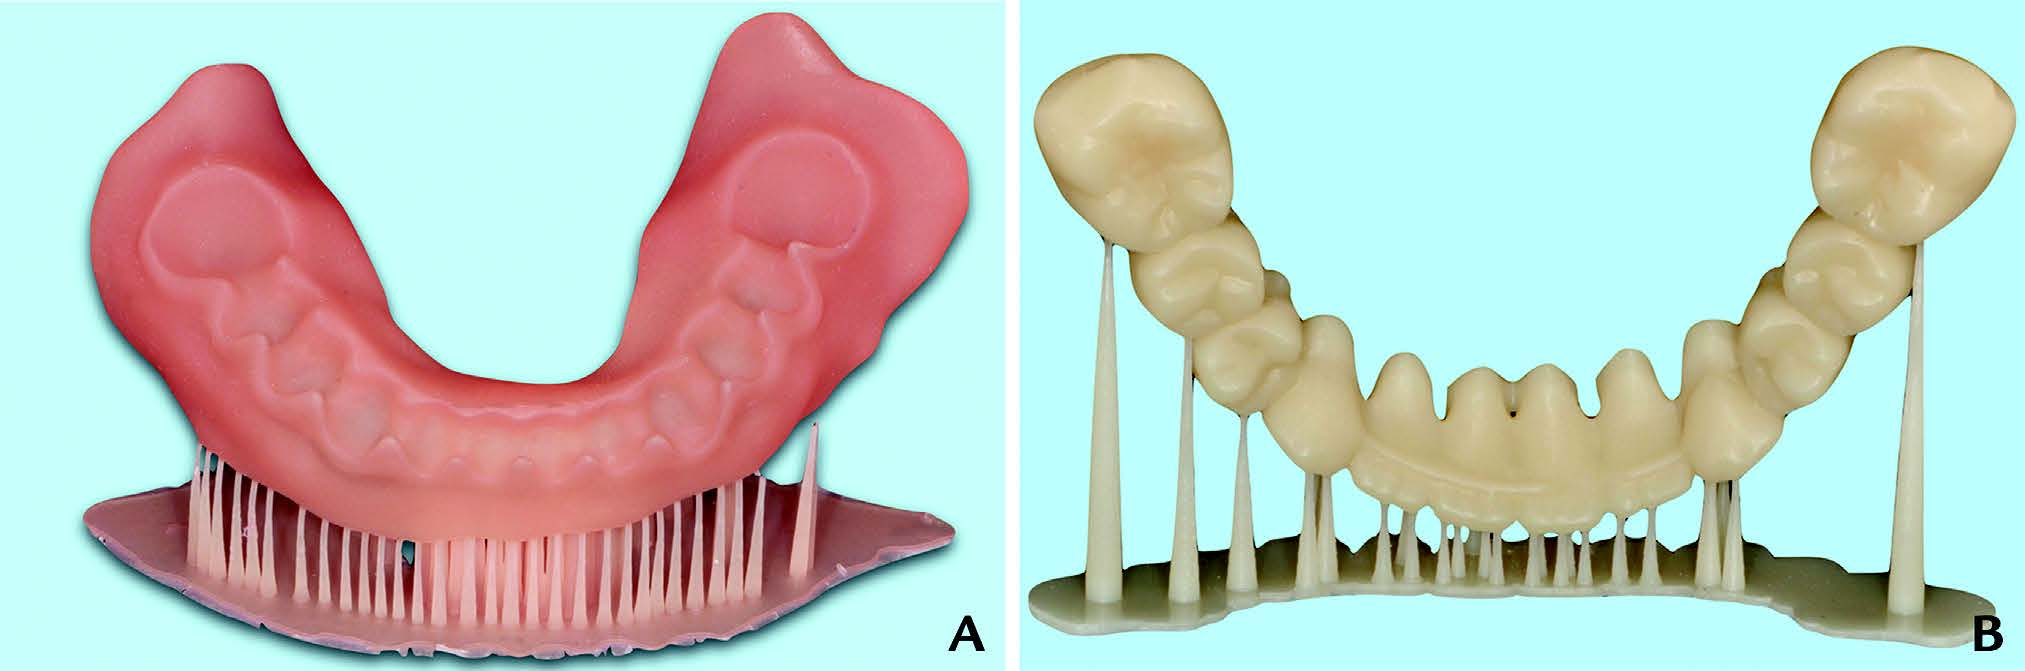
\includegraphics[width=0.9\textwidth,height=\textheight,keepaspectratio]{separ_full_prot}
    \caption{Componenti di Protesi mobile totale provvisoria realizzati con design digitale e stampante 3D DLP. Da \emph{Lin et al} \parencite{Reference108}}
    \label{fig:separ_full_prot}
    \end{center}
\vspace{-30pt}
\end{figure}

\subsection{Ortodonzia} 
Orthodontics is one of the branches of dentistry that can best avail itself of the new possibilities of digital programming of treatment and the use of additive manufacturing technologies. Orthodontic therapy is classically programmed by means of teleradiographs, plaster models in the articulator and set of photos of the patient, in addition to the fundamental clinical and functional evaluation. The complex relationships between the bones of the skull involved in the oral function are difficult to analyze adequately on two-dimensional radiographs and with plaster models, especially if the treatment involves a surgical phase.\\
Digital orthodontic therapy can use the ability to print custom brackets \parencite{Reference115} and surgical guides for the insertion of orthodontic implants \parencite{Reference116} \ref{fig:stent_miniscrew}. 3D printing also facilitates the production of guides for positioning brackets in the patient \parencite{Reference127}, which favor a fast and precise positioning of the same, and of personalized auxiliary tools \parencite{Reference126}. The custom brackets were made by Krey through FreeCAD software and a DLP printing process \ref{fig:design_brackt}. With the same technique a positioning splint was printed, previously designed virtually, which allowed to position the brackets quickly and precisely. Intraoral scans at time intervals were performed and compared in MeshLab to verify the orthodontic movement of the dental elements; the post treatment retention splint was also virtually designed and printed in 3D. \\
\begin{figure}[h!]
 
\begin{subfigure}{0.5\textwidth}
\centering
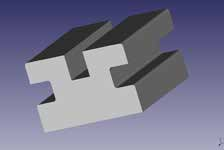
\includegraphics[width=0.9\linewidth, keepaspectratio]{design_brackt} 
\caption{Design CAD del bracket.}
\label{fig:design_brackt}
\end{subfigure}
\begin{subfigure}{0.5\textwidth}
\centering
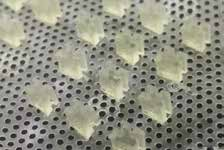
\includegraphics[width=0.9\linewidth, keepaspectratio]{printd_brackt}
\caption{Brackets stampati.}
\label{fig:printd_brackt}
\end{subfigure}
\begin{subfigure}{0.5\textwidth}
\centering
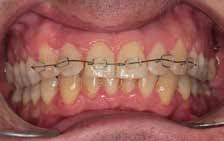
\includegraphics[width=0.9\linewidth, keepaspectratio]{working_brackt}
\caption{Brackets stampati in funzione all'interno del cavo orale.}
\label{fig:working_brackt}
\end{subfigure}
\begin{subfigure}{0.5\textwidth}
\centering
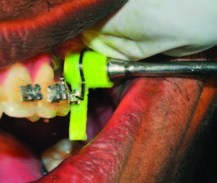
\includegraphics[width=0.7\linewidth, keepaspectratio]{stent_miniscrew}
\caption{Guida per l'inserimento di impianti ortodontici stampata in 3D}
\label{fig:stent_miniscrew}
\end{subfigure}
\caption{A, B e C da \emph{Krey et al} \parencite{Reference115}, D da \emph{Ahamed et al} \parencite{Reference116}}
\label{fig:3d_ortho}
\end{figure}

This was a test study with brackets \emph{edgewise} molded in light-curable resin; the authors suggested the possibility of revising part of the design to optimize the resistance of the brackets. The report is generally positive and opens up the possibility of a radical change in the way in which orthodontics with fixed devices can be performed in the dental office, with the transition from the use of generic brackets to custom brackets achievable in the clinic.
In modern dental practice, the use of plaster models is often accompanied by digital scans and 3D printing of the model. Several authors have evaluated the accuracy of models made with additive manufacturing techniques, with different results. Dietrich \parencite{Reference112} evaluated the accuracy and accuracy of dental models made with polyjet and SLA techniques. The printed models were scanned and evaluated via software to evaluate the discrepancy with the original. Both methods of printing proved to be capable of printing accuracy suitable for orthodontic use, with a maximum detected error of about \SI{100}{\micro\metre}. \\
Wan Hassan \parencite{Reference113} manually compared, by means of a caliber, dental arched models of patients, made of plaster and printed with SLA technology. The author has decreed the models not suitable for orthodontic use due to a discrepancy of about 1mm compared to the original. The author reports that the digital scanning of the plaster models resulted in a loss of detail, moreover the measurements with gauge were sometimes not easy to carry out due to the overcrowding. Both of these conditions may have contributed to the reported error. Removable devices can also be manufactured with 3D printing \parencite{Reference111}. In addition, 3D printed surgical guides have been used to perform cortical osteotomies in order to accelerate orthodontic movements \parencite{Reference114}. \\
The possibility of integration that digital orthodontics also allows us from the biomechanical point of view is very important. The use of optical scans and CBCT allows detailed information on the patient's structure. Orthodontic movements are based on biological and physical principles, where controlled forces are used to activate the bone remodeling process, which allows the movement of the dental element. These factors could be investigated by integrating the anatomical data (bones, muscles, ligaments, organs) and functional data (masticatory force, mechanical characteristics of the tissues and materials involved, range of mandibular movement \ldots) to simulate in silico treatment, providing to the patient a personalized treatment according to its biological and response characteristics \parencite{Reference110}, \parencite{Reference140}.
\begin{figure}[h]
\vspace{-10pt}
	\begin{center}
	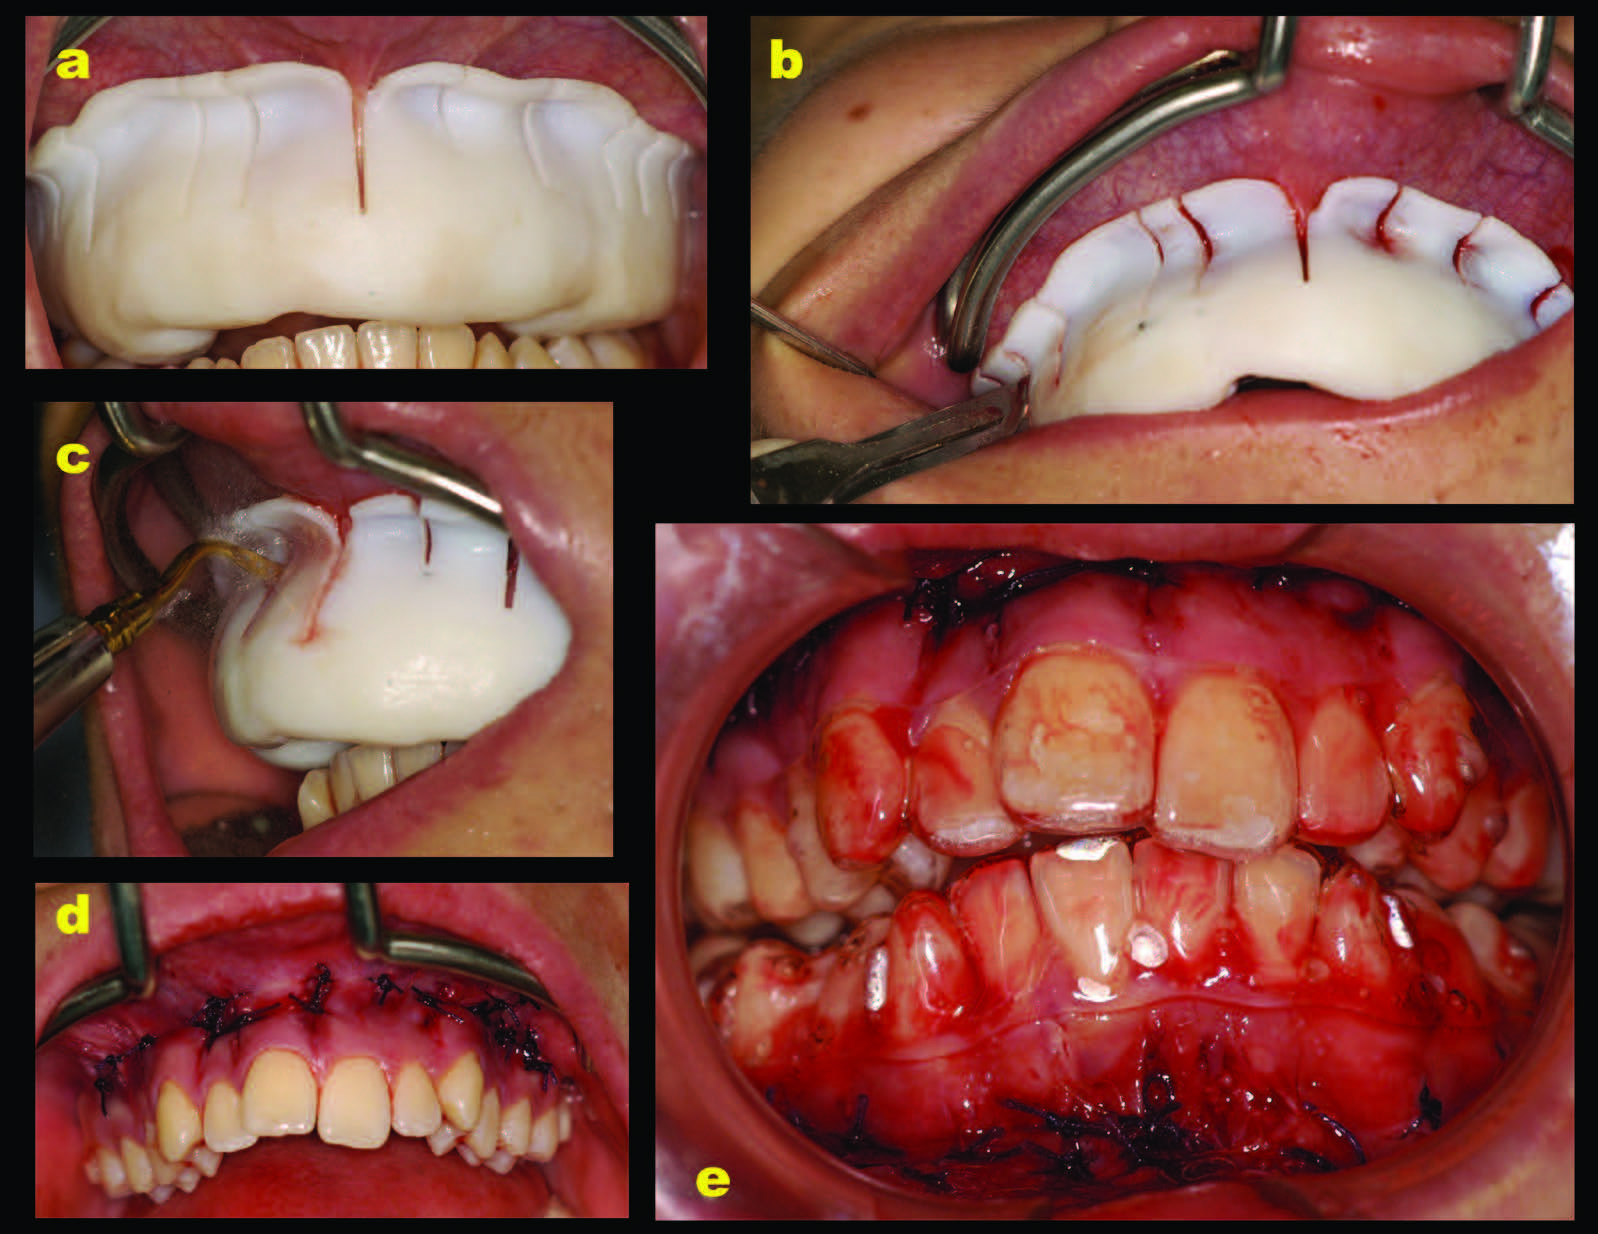
\includegraphics[width=0.9\textwidth, keepaspectratio]{guide}
    \caption{Posizionamento della guida chirurgica stampata in 3D per l'esecuzione di osteotomie flapless. \textbf{a}: Valutazione della stabilità intraorale. \textbf{b}: incisioni verticali della gengiva con bisturi n15. \textbf{c}: corticotomie verticali eseguite usando uno strumento piezoelettrico. \textbf{d}: sutura delle incisioni. \textbf{e}: posizionamento degli allineatori trasparenti dopo la chirurgia. Da \emph{Cassetta et al} \parencite{Reference114}.}
    \label{fig:guide}
	\end{center}
\vspace{-20pt}
\end{figure}

 
 